\documentclass[a4paper]{book}
\usepackage[UTF8]{ctex}
\usepackage{tikz}\usetikzlibrary{arrows,calc,intersections,through,backgrounds,math,angles,shapes}
\usepackage{hyperref}
\usepackage{amsmath,amssymb,mathrsfs}
\usepackage[includemp=true,marginparsep=.5cm,marginparwidth=3cm,left=2.5cm,right=2cm]{geometry}%带旁注
\def\sky{\par\vspace*{1ex}}
\newcommand\tbs[1][]{\tt\char`\\#1}
\newcommand\Dd{\displaystyle}
\newcommand\bpics[1]{\par\vspace{1ex}\noindent\begin{minipage}{\textwidth}\begin{minipage}{#1\textwidth}}
\newcommand\mpics[1]{\end{minipage}\begin{minipage}{#1\textwidth}\linespread{1}}
\newcommand\epics{\end{minipage}\end{minipage}\par\vspace{2ex}}
\begin{document}
\tableofcontents
\chapter{基础知识}




\chapter{表格处理}
\chapter{编绎}
\chapter{宏包介绍}
\section{xcolor}
定义颜色\verb|\definecolor{bgcolor-co}{RGB}{255,255,255}|

    \begin{description}
        \item[红色] 一种激奋的色彩。刺激效果,能使人产生冲动,愤怒,热情,活力的感觉。
        \item[绿色] 介于冷暖两中色彩的中间,显得和睦,宁静,健康,安全的感觉。它和金黄,淡白搭配,可以产生优雅,舒适的气氛。
        \item[橙色] 也是一种激奋的色彩,具有轻快,欢欣,热烈,温馨,时尚的效果。
        \item[黄色] 具有快乐,希望,智慧和轻快的个性,它的明度最高。
        \item[蓝色] 是最具凉爽,清新,专业的色彩。它和白色混合,能体现柔顺,淡雅,浪漫的气氛 (像天空的色彩:)
        \item[白色] 具有洁白,明快,纯真,清洁的感受。
        \item[黑色] 具有深沉,神秘,寂静,悲哀,压抑的感受。
        \item[灰色] 具有中庸,平凡,温和,谦让,中立和高雅的感觉。
    \end{description}

    \newcommand\colorect[2]{\fill[#1](#2)node[above=4pt,right=1pc,black]{#1}rectangle+(1pc,0.618pc);}
    \subsubsection{基本颜色}
        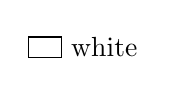
\begin{tikzpicture}
            \colorect{black}{0,1.5}   \colorect{blue}{0,1}   \colorect{brown}{0,.5} \colorect{cyan}{0,0}
            \colorect{darkgray}{2,1.5}\colorect{gray}{2,1}   \colorect{green}{2,.5} \colorect{lightgray}{2,0}
            \colorect{lime}{4,1.5}    \colorect{magenta}{4,1}\colorect{olive}{4,.5} \colorect{orange}{4,0}
            \colorect{pink}{6,1.5}    \colorect{purple}{6,1} \colorect{red}{6,.5}   \colorect{teal}{6,0}
            \colorect{violet}{8,1.5}  \colorect{yellow}{8,.5} \filldraw[draw=black,fill=white](8,1)node[above=4pt,right=1pc,black]{white}rectangle+(1pc,0.618pc);
        \end{tikzpicture}
    \subsubsection{green!60!white}
        \newcommand\colorecti[3]{\fill[#1](#3)node[above=4pt,right=1pc,black]{#2}rectangle+(1pc,0.618pc);}
        \newcommand\colorsix[3]{\colorecti{#1!100!#2}{#1}{#3,2.5}\colorect{#1!80!#2}{#3,2}\colorect{#1!60!#2}{#3,1.5}%
          \colorect{#1!40!#2}{#3,1}\colorect{#1!20!#2}{#3,.5}\colorecti{#1!0!#2}{#2}{#3,0}}%
        \begin{tikzpicture}
            \colorsix{green}{white}{0}
            \colorsix{green}{gray}{4}
            \colorsix{green}{black}{8}
        \end{tikzpicture}\sky\sky
        \begin{tikzpicture}
            \colorsix{green}{red}{0}
            \colorsix{green}{blue}{4}
            \colorsix{green}{yellow}{8}
        \end{tikzpicture}
        \subsubsection{多色混合}
            \begin{tikzpicture}
                \colorect{red}{0,3}  \colorecti{-red!100}{-red}{6,3}
                \colorect{red!75}{0,2.5}  \colorect{-red!75}{6,2.5}
                \colorect{red!75!green}{0,2}  \colorect{-red!75!green}{6,2}
                \colorect{red!75!green!50}{0,1.5}  \colorect{-red!75!green!50}{6,1.5}
                \colorect{red!75!green!50!blue}{0,1}  \colorect{-red!75!green!50!blue}{6,1}
                \colorect{red!75!green!50!blue!25}{0,.5}  \colorect{-red!75!green!50!blue!25}{6,.5}
                \colorect{red!75!green!50!blue!25!gray}{0,0}  \colorect{-red!75!green!50!blue!25!gray}{6,0}
            \end{tikzpicture}
    \subsection{PGF}
        宏包调用的名称是 tikz

        PGF的缺省长度单位的 1cm
        \begin{verbatim}
          \pgfsetxvec{\pgfpoint{10pt}{0}}
          \pgfsetyvec{\pgfpoint{0pt}{10pt}}
        \end{verbatim}
\section{paralist}
  \LaTeX 的列表缺省行间距较大,如要节省空间,可以考虑 Bernd Schandl的 paralist 宏包,它提供了一系列压缩列表和行间列表环境。

  它提供了类似的环境 compactitem, compactenum, compactdesc. 另外还提供了行间列表环境 inparaitem, inparaenum, inparadesc.
\end{document} 
